\section{システム}


\subsection{ハードウェア}
自律走行を行う機体で必要な要素は大きく分けると下記5点となる。

\begin{itemize}
    \item センサ
    \item 走行装置
    \item 計算機
    \item バッテリー
    \item シャーシ
\end{itemize}

この章では、搭載したハードウェアがどのように使用されたか説明する。

\subsubsection{自律走行ロボット:Penguin}
今回、自律走行を実現する基本的な構成を持ちつつ、不整地の走行も可能な機体とすることをコンセプトに、機体を作成した。 
作成した機体とその搭載した機器を、図\ref{fig:robot}に記載する。この章では、各要素について詳細を説明する。

\subsubsection{センサ}
Penguinには、エンコーダ、IMU、LiDARの3種類のセンサが搭載されている。

エンコーダはモータの回転数を計測するもので、どのくらいモータが回転したか累積を数えることでロボットのホイールオドメトリを推定する。
ただし、スリップや量子化誤差などで誤差が蓄積するためこの値をそのまま使用することはできない。
後述のLiDARを使って外界の情報を得ることで補正して使用した。

IMUはロボットのX、Y、Z方向の加速度とRoll、Pitch、Yaw方向の角加速度を取得できる。
この値を累積することで、ジャイロオドメトリを推定することができる。
ホイールオドメトリのようにスリップすることはないが、段差などの影響を強く受ける。
今回は、SLAMアルゴリズムでの位置補正に使用した。

LiDARは距離を知ることができるセンサである。
今回搭載したLiDARは3DLiDARで、ロボット周辺の形状を3次元の点群として得ることができる。
3DLiDARは自己位置推定用のものと、障害物認識用のものの2つを搭載した。

自己位置推定を行うためのLiDARセンサとして、Velodyne社のVLP-16\cite{VLP16}を搭載した。
VLP-16は100mという長距離の測定が可能であるため、つくば市庁舎やつくばエクスプレスの建物を常に観測できる。
ロボット近傍で人だかりができて周囲の景気が見えづらくなっても、自己位置推定を維持しやすい。
なるべく周囲の物体によってLiDARの光を阻害されないように機体の最上部に搭載した。
また、非常に高額なセンサであるため、転倒したり、ものが当たって傷つかないように金蔵製のガードも合わせて設置した。

障害物を検出するLiDARとして、Livox社のMID-360\cite{MID360}を搭載した。
MID-360はVLP-16のような長距離の物体を測定することはできないが、非常に密な空間測距ができる。
また、FoVも60度と広く、ロボットに衝突しそうな近くの物体を精細に取られることができるLiDARである。

障害物検知用のLiDARは、接近する物体を検知するため、機体の下部に設置し、35度下向きに傾けて設置した。
これにより、ロボットの前方250mmの地面を測距できるため、衝突しそうになるギリギリまでの距離の物体を測定できる。
また、今回の機体は後進を行わないため、障害物の検出範囲は前方向のみとした。
障害物検出用のLiDARも、光学窓への傷を防ぐため金属製のガードを上下に設置した。

\subsubsection{走行装置}
走行装置には、CuboRex社のクローラロボット開発プラットフォーム CuGo V4\cite{CuGo}を使用した。
不整地走行に適したクローラを有するプラットフォームを使用する事で、不整地の走破性向上と開発の高速化を図った。

\subsubsection{計算機}
ロボットの制御を行うPCとして、ASUS社のROG Strix SCAR 15 G532LWS\cite{PC}を搭載した。
ノートPCを搭載することにより、ロボットを駆動する電源系列とPCを駆動する計算機の電源分割を実現した。

モータの制御には、CuboRex社製モータドライバに付属しているRaspberry Pi Pico\cite{PICO}を使用した。

\subsubsection{バッテリー}
機体下部に、24V20Ah のLiFePO4バッテリを搭載した。
本機体は不整地走行の可能性を考慮し、LiPoバッテリより安全性の高いLiFePO4バッテリーを採用した。

バッテリは機体下部に設置することで、重心の上昇による安定性の低下を防いだ。
バッテリから供給される電源は、ロボットに搭載した電源分配基板により適切に切替・分配・変圧し、PCを除く各機器に接続した。

\subsubsection{シャーシ}
屋外でのデバッグ作業を想定し、日よけの壁を搭載した。
ロボットは図\ref{fig:decomposition}のような5ユニットで構成し、各部を計10本のボルトで分解できる形とした。
分解箇所には付当てを設置し、複数回の分割、組立を実施しても再現性のあるシャーシとなる形とした。

構造部材にはミスミ社 R形状アルミフレーム\cite{MISUMI}を使用することで、衝突しても対象に危害を加えにくい形状を実現した。
突起部・巻き込みが発生しうる箇所には、樹脂製のカバーを搭載した。

ロボットの状態表示のため、アルミフレームの溝部にLEDを搭載した。
このLEDの色でロボットが自律走行状態か、操作者による操作を実施している状態かを一般通行者に対して示した。



\subsection{ソフトウェア}
ロボットを走行させるためのソフトウェア構成は以下の通りである。
\begin{itemize}
    \item 地図作成
    \item 自己位置推定
    \item 障害物認識
    \item 経路計画
    \item 経路追従
\end{itemize}

自律走行を実現するために、上記のタスクを同時に満たすナビゲーションシステムを構築した。
図\ref{fig:system}にナビゲーションシステムの概要を示す。
このシステムを構築するために多くはOSSであるROS 2\cite{ROS2}を使用した。
このレポートでは、上記のそれぞれのタスクについてどのようなアプローチをしたか述べる。

本システムで自律走行をするためには走行する範囲の地図を作成する。
現実の場所とリンクした地図をロボットに持たせることでロボットが目的地と現在地の相対位置把握することができる。
このロボットに持たせる地図の精度が後述の自己位置推定の精度に大きな影響を与えるため、効率的で精度の高い地図を作成することが大事である。
この地図作成は第3章で説明する。

次に、ロボットの現在位置を推定する。LiDARなどのセンサ情報から自分自身が地図上のどの位置にいるのかを推定する。
現在位置が分かれば、目的までの向かう経路を計算することができる。
正確な位置情報を維持し続けるために3Dの地図から回転式3DLiDARのセンサ値とオドメトリ情報を使用して自己位置推定を行う方法を第4章で説明する。

自己位置推定ができても、実際には障害物があってたどり着かないことがほとんどである。
向かいたい場所までの経路上に障害物がどのようにあるのか反映させる。
ロボット直近の広範囲で高密度な点群を取得できる3DLiDARを使用して、2DLiDARでは見逃しがちな細長い物体を検知し、坂道などの検知したくない物体を除外することができた。
この障害物検知手法は第5章で説明する。

ロボットの現在位置と障害物を知ることができると、目的地までの障害物を避けた経路を計算することができる。
実際の自律走行では、スタート地点から本走行のゴール地点まで1度に経路を計算しない。
数メートルおきに小さなゴール地点を作成し、そこに到達することを繰り返す。
経路を計算した後には、ロボットがこの経路を正確にトレースするようにアクチュエータの出力を制御する。
しかし、線路の上を電車が走行するように、計算した経路を忠実に走行すれば良いとは言えない。
ロボットハードの都合で急停止や急旋回が物理的に実現できなかったり、とっさに現れた障害物を回避する必要があるためである。
障害物を回避しながら、必要十分に経路をなぞる制御を経路追従という。
第6章では、経路計画と経路追従を行うナビゲーションについて説明する。

最後に、本走行の結果と今後の展開について述べる。

\begin{figure*}[htbp]
    \centering
    \begin{minipage}[b]{0.45\hsize}
       \centering
       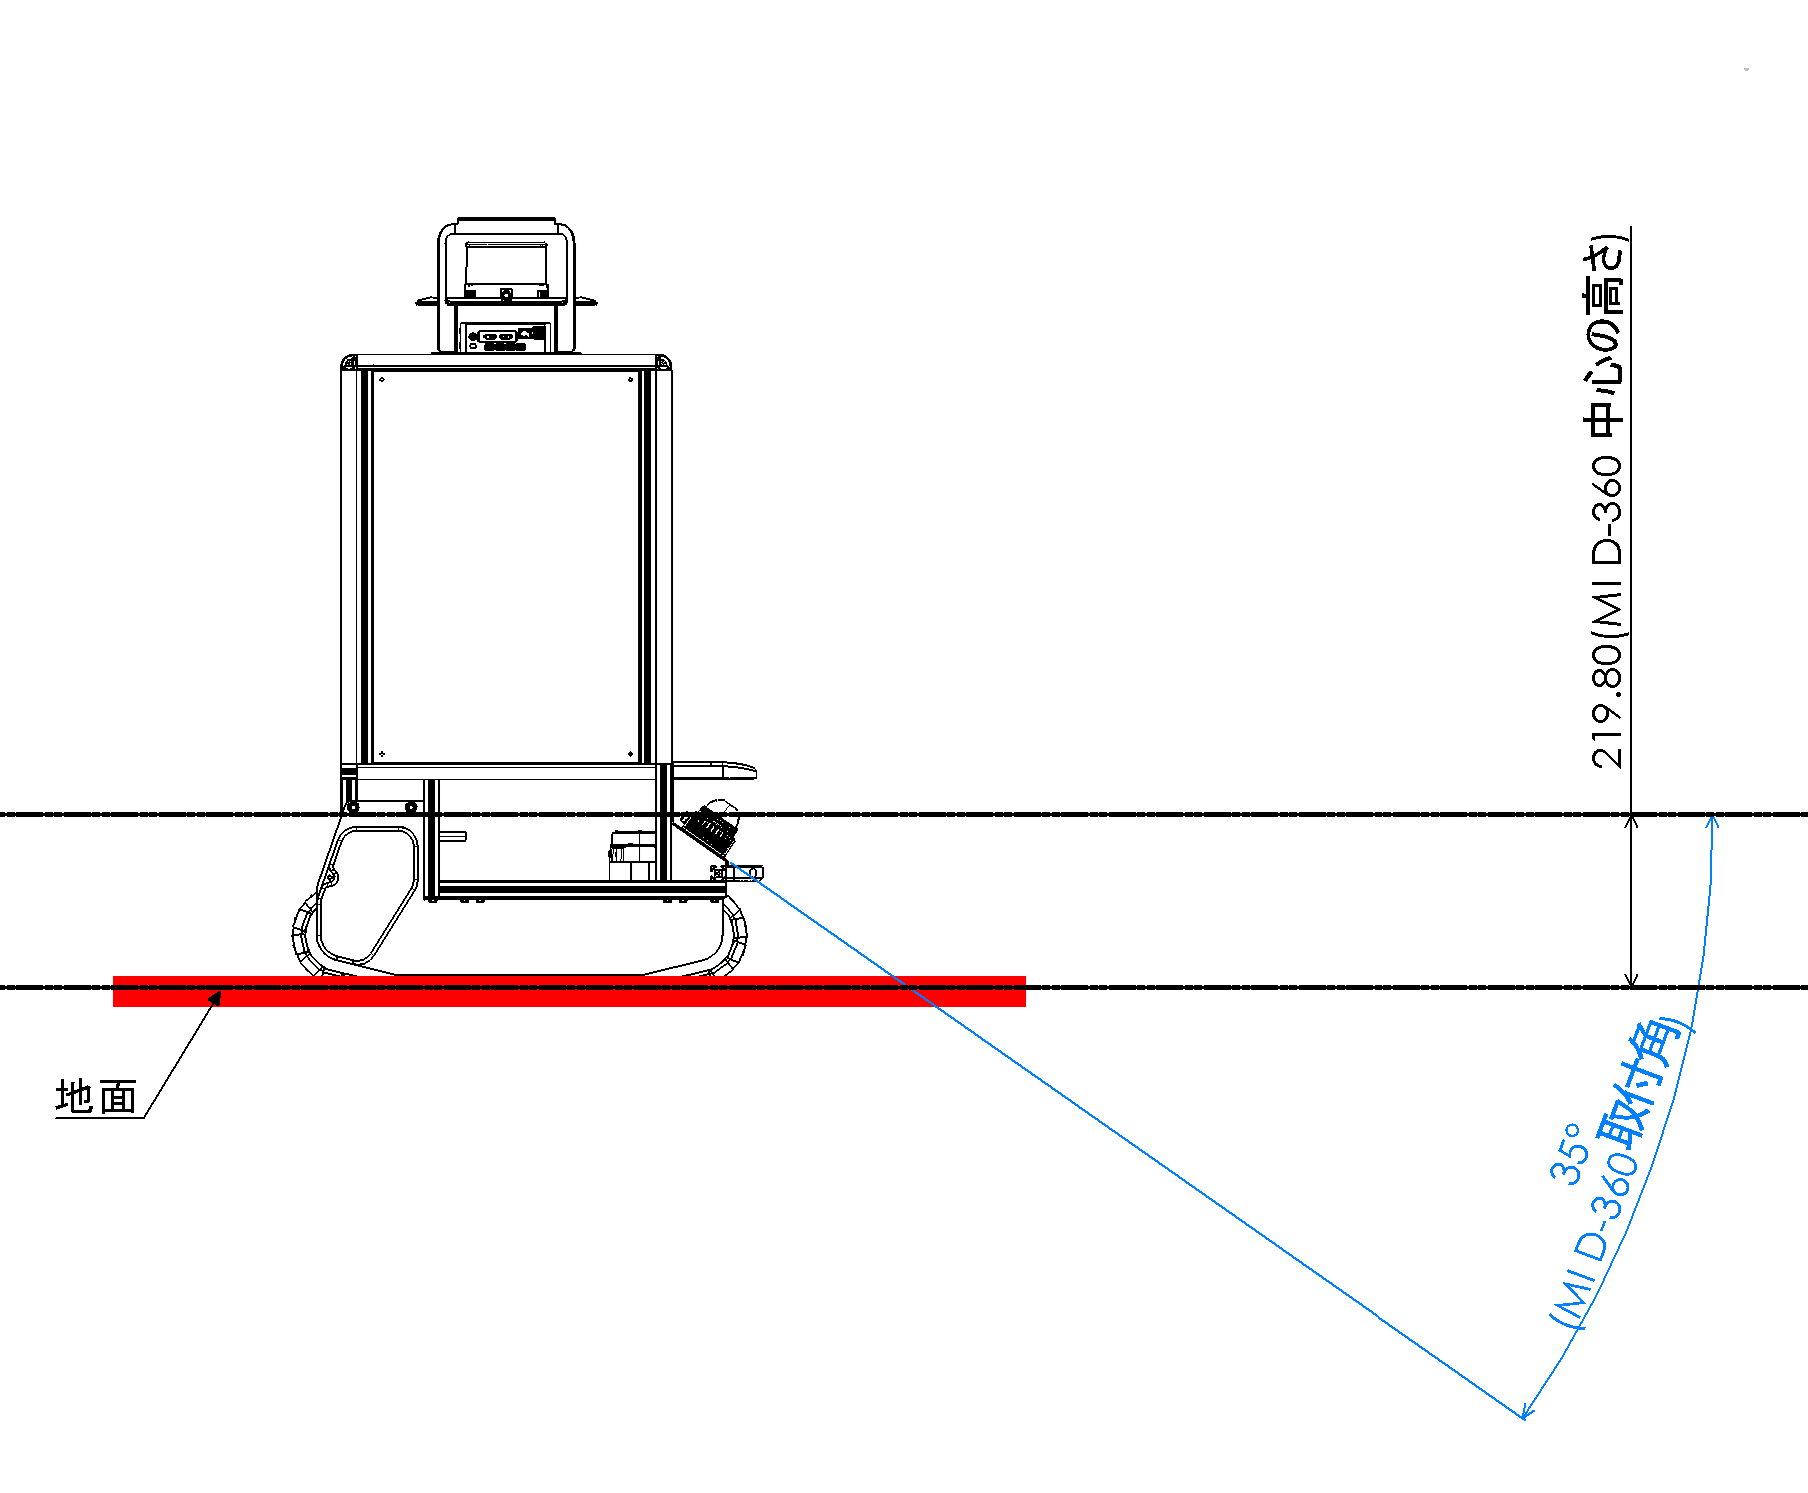
\includegraphics[height=5cm]{fig/obstacle_detection_range_sideview.png}
       \caption{障害物検知用のLiDAR取り付け位置}
       \label{fig:detection}
    \end{minipage}
  %
    \begin{minipage}[b]{0.45\hsize}
       \centering
       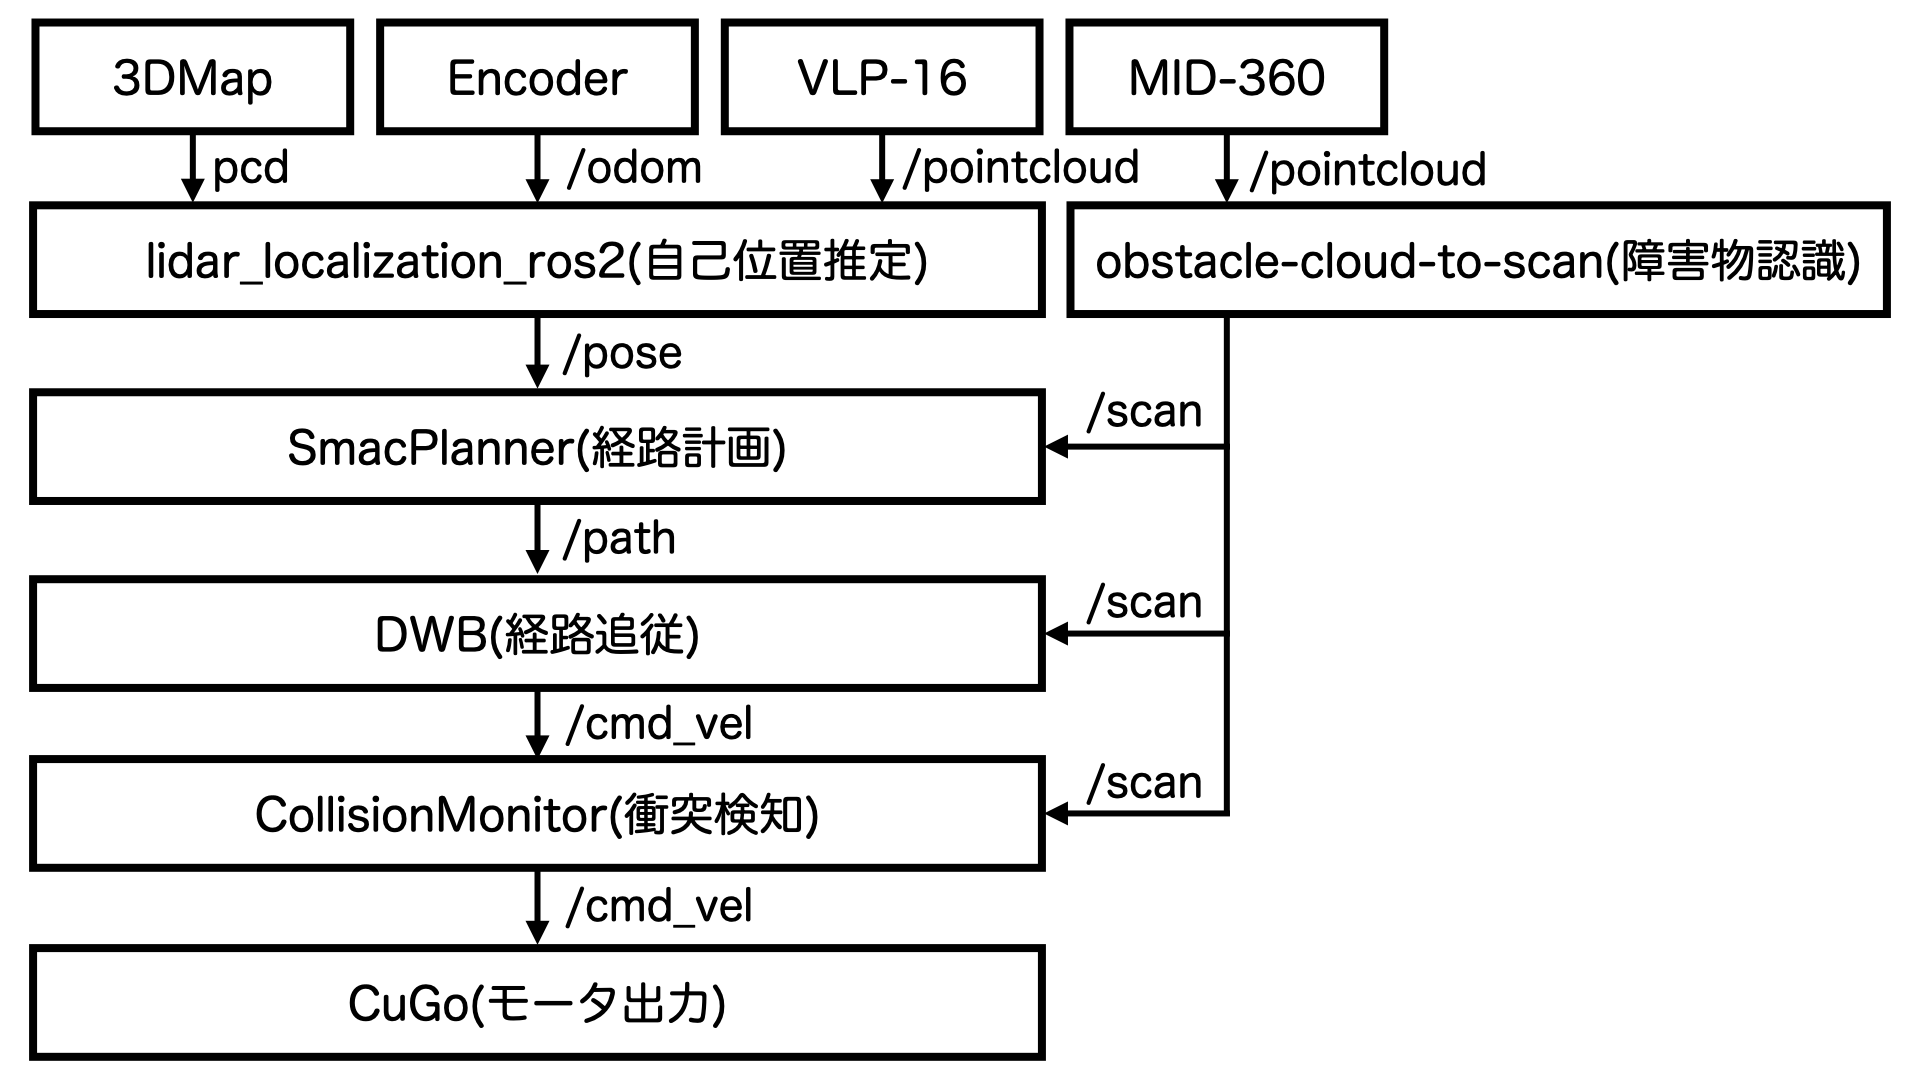
\includegraphics[height=5cm]{fig/system.png}
       \caption{ナビゲーションシステムの構成}
       \label{fig:system}
    \end{minipage}
\end{figure*}